\chapter{Einleitung} 

Durch längere Lagerung und thermische Belastung kann in Honig Hydroxymethylfurfural (HMF) in größerer Konzentration entstehen. HMF steht im Verdacht krebserregend zu sein. Zudem ist ein niedriger Gehalt an HMF ein Indikator für die Frische und Naturbelassenheit von Honig.
\begin{figure}[htbp]
	\centering
		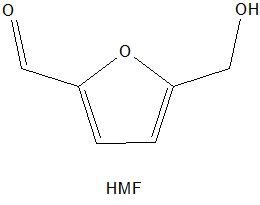
\includegraphics[width=0.5\textwidth]{../Bilder/HMF.jpg}
	\caption{Hydroxymethylfurfural}
	\label{fig:HMF}
\end{figure}
\newline
Eine Möglichkeit das HMF in Honig zu bestimmen ist die photometrische Methode nach WINKLER. Mittels einer Farbreaktion wird ein rot erscheinender Farbstoff erzeugt, der anschließend quantifiziert wird. Zur  Bestimmung des HMF-Gehalts wird zunächst die Methode, wie in dem Buch Lebensmittelanalytik~\cite{Lebensmittelanalytik} beschrieben, nachgestellt. Da in der zur Verfügung stehenden Methode lediglich ein Festfaktor zur Quantifizierung angegeben ist wird zusätzlich eine Kalibrierreihe mit mehreren Punkten durchgeführt. Des weiteren wird die Methode auf Reproduzierbarkeit überprüft. Zur Ermittlung des Massenanteils an HMF sollen mehrere Arten der Quantifizierung verwendet werden. Diese sind zum einen die Berechnung über den angegebenen Festfaktor, die Verwendung der erstellten Kalibriergerade sowie über Aufstockung einer Probe mit anschließender Standardaddition. Es werden acht verschiedene Honige, ein Rübensirup und eine Invertzuckermischung, die bei Raumtemperatur aufbewahrt wurden, vermessen. Außerdem werden sechs Honige für zehn Tage bei $60^\circ$ C gelagert um einen Anstieg des HMF-Gehalts nachzuweisen. Die Handhabung der Proben ist durch ihre Viskosität erschwert. Da der Honig viele verschiedene, zum Teil unlösliche Bestandteile enthält, wird diese Matrix vor der Bestimmung entfernt. Die verwendeten Chemikalien erfordern auf Grund ihrer gefährlichen Eigenschaften eine besondere Sorgfalt bei der Handhabung. Ihre Haltbarkeit ist auch bei korrekter Lagerung sehr begrenzt. Der bei der Durchführung entstandene Farbstoff ist nicht stabil und zerfällt wenige Minuten nach der Aufarbeitung. Deshalb muss jede Lösung zeitlich exakt vermessen werden.~\cite{Winkler}